\chapter{Specifikacija programske potpore}
		
	\section{Funkcionalni zahtjevi}
			
			\textbf{\textit{dio 1. revizije}}\\
			
			\textit{Navesti \textbf{dionike} koji imaju \textbf{interes u ovom sustavu} ili  \textbf{su nositelji odgovornosti}. To su prije svega korisnici, ali i administratori sustava, naručitelji, razvojni tim.}\\
				
			\textit{Navesti \textbf{aktore} koji izravno \textbf{koriste} ili \textbf{komuniciraju sa sustavom}. Oni mogu imati inicijatorsku ulogu, tj. započinju određene procese u sustavu ili samo sudioničku ulogu, tj. obavljaju određeni posao. Za svakog aktora navesti funkcionalne zahtjeve koji se na njega odnose.}\\
			
			
			\noindent \textbf{Dionici:}
			
			\begin{packed_enum}
				
				\item Organizator konferencije (naručitelj)
				\item Pokrovitelji konferencije
				\item Autori radova
				\item Glasači
				\item Administrator
				\item Razvojni tim
				
			\end{packed_enum}
			
			\noindent \textbf{Aktori i njihovi funkcionalni zahtjevi:}
			
			\begin{packed_enum}
				\item  \underbar{Neregistrirani/Neprijavljeni korisnik (inicijator) može:}
				
				\begin{packed_enum}
					
					\item upisati lozinku za konferenciju
					\item registrirati se to jest stvoriti novi korisnički račun za koji su mu potrebni: korisničko ime, lozinka i adresa e-pošte
					\item prijaviti se
					\item pregledavati postere, pri čemu ne može glasati
					
				\end{packed_enum}
			
				\item  \underbar{Registrirani/Prijavljeni korisnik (inicijator) može:}
				
				\begin{packed_enum}
					
					\item pregledavati i mijenjati osobne podatke
					\item izbrisati svoj korisnički račun
					\item pregledavati i glasati za postere pri čemu svaki posjetitelj može glasati najviše za jedan poster
					\item pregledavati promotivne materijale pokrovitelja
					\item gledati video-prijenos
					\item pregledavati i preuzimati fotografije
					\item vidjeti informacije o mjestu održavanja koje uključuju vremenske uvjete i vremensku prognozu
					\item pristupiti rezultatima jednom kad postanu dostupni
				
				\end{packed_enum}
				
				\item \underbar{Administrator (inicijator) može:}
				
				\begin{packed_enum}
					
					\item prijaviti i ukloniti autore, radove i postere
					\item pristupiti svim podacima
					\item definirati sve uvjete za rad sustava
					
				\end{packed_enum}
				
				\item \underbar{Baza podataka (sudionik):}
				
				\begin{packed_enum}
					
					\item pohranjuje podatke o korisnicima
					\item pohranjuje podatke o digitalnim posterima, broju njihovih glasova, njihovim autorima
					\item pohranjuje fotografije uslikane za vrijeme trajanja konferencije
					
				\end{packed_enum}
				
				\item \underbar{Poslužitelj strujanja (sudionik):}
				
				\begin{packed_enum}
					
					\item pruža uslugu video prijenosa konferencije
				
				\end{packed_enum}
				
				\item \underbar{Poslužitelj podataka o vremenu (sudionik):}
				
				\begin{packed_enum}
					
					\item poslužuje potrebne podatke vezane za prognozu vremena
					
				\end{packed_enum}
				
				\item \underbar{Poslužitelj e-pošte (sudionik):}
				
				\begin{packed_enum}
					
					\item omogućuje aplikaciji da šalje e-poruke korisnicima
					
				\end{packed_enum}
				
			\end{packed_enum}
			
			\eject 
			
			
				
			\subsection{Obrasci uporabe}
				
				\textbf{\textit{dio 1. revizije}}
				
				\subsubsection{Opis obrazaca uporabe}
					\textit{Funkcionalne zahtjeve razraditi u obliku obrazaca uporabe. Svaki obrazac je potrebno razraditi prema donjem predlošku. Ukoliko u nekom koraku može doći do odstupanja, potrebno je to odstupanje opisati i po mogućnosti ponuditi rješenje kojim bi se tijek obrasca vratio na osnovni tijek.}\\
					
					\newcounter{UseCaseCounter}
					\setcounter{UseCaseCounter}{1}
					
					%UC1
					\noindent \underbar{\textbf{UC\theUseCaseCounter \stepcounter{UseCaseCounter} - Pristup konferenciji}}
					\begin{packed_item}
	
						\item \textbf{Glavni sudionik: } Neprijavljeni korisnik
						\item  \textbf{Cilj:} Pristup konferenciji
						\item  \textbf{Sudionici:} Baza podataka
						\item  \textbf{Preduvjet:} Korisnik već nije prijavljen
						\item  \textbf{Opis osnovnog tijeka:}
						
						\item[] \begin{packed_enum}
	
							\item Korisnik pokreće aplikaciju
							\item Pojavljuje se obrazac za upis lozinke za pristup konferenciji (isti je za sve korisnike za tu konferenciju)
							\item Korisnik upiše lozinku te ju potvrđuje
							\item Obrazac za upis lozinke nestaje i pojavljuje se ekran s prikazom svih postera
						\end{packed_enum}
						
						\item  \textbf{Opis mogućih odstupanja:}
						
						\item[] \begin{packed_item}
	
							\item[3.a] Korisnik upiše krivu lozinku
							\item[] \begin{packed_enum}
								
								\item Pristup pregledu konferencije je odbijen
								\item Sustav obavještava korisnika o upisu pogrešne lozinke ili imena
								
							\end{packed_enum}
							
						\end{packed_item}
					\end{packed_item}
					
					%UC2
					\noindent \underbar{\textbf{UC\theUseCaseCounter \stepcounter{UseCaseCounter} - Prijava}}
					\begin{packed_item}
						
						\item \textbf{Glavni sudionik: } Neprijavljeni korisnik
						\item  \textbf{Cilj:} Pristup svim korisničkim funkcionalnostima aplikacije
						\item  \textbf{Sudionici:} Baza podataka
						\item  \textbf{Preduvjet:} Korisnik je registriran
						\item  \textbf{Opis osnovnog tijeka:}
						
						\item[] \begin{packed_enum}
							
							\item Korisnik pritišće gumb za prijavu na početnoj stranici
							\item Otvara se novi prozor u koji korisnik upisuje podatke
							\item Provjera postoji li korisnik u bazi podataka
							\item Ako korisnik postoji, otvara se prozor s posterima, a korisnik je prijavljen
						\end{packed_enum}
						
						\item  \textbf{Opis mogućih odstupanja:}
						
						\item[] \begin{packed_item}
							
							\item[4.a] Korisnik ne postoji u bazi podataka
							\item[] \begin{packed_enum}
								
								\item Sustav obavještava korisnika o upisu pogrešne lozinke ili imena
								
							\end{packed_enum}
							
						\end{packed_item}
					\end{packed_item}	
					
					%UC3
					\noindent \underbar{\textbf{UC\theUseCaseCounter \stepcounter{UseCaseCounter} - Registracija}}
					\begin{packed_item}
					
						\item \textbf{Glavni sudionik: } Neprijavljeni korisnik
						\item  \textbf{Cilj:} Stvoriti korisnički račun za pristup sustavu
						\item  \textbf{Sudionici:} Baza podataka
						\item  \textbf{Preduvjet:} Korisnik je pristupio konferenciji 
						\item  \textbf{Opis osnovnog tijeka:}
						
						\item[] \begin{packed_enum}
							
							\item Korisnik odabire opciju za registraciju
							\item Korisnik unosi potrebne korisničke podatke
							\item Korisnik prima obavijest o uspješnoj registraciji

						\end{packed_enum}
						
						\item  \textbf{Opis mogućih odstupanja:}
						
						\item[] \begin{packed_item}
							
							\item[2.a] Odabir već zauzetog korisničkog imena i/ili e-maila, unos korisničkog podatka u nedozvoljenom formatu ili pružanje neispravnog e-maila
							\item[] \begin{packed_enum}
								
								\item Sustav obavještava korisnika o neuspjelom upisu i vraća ga na stranicu za registraciju
								\item Korisnik mijenja potrebne podatke te završava unos ili odustaje od registracije
								
							\end{packed_enum}
							
						\end{packed_item}
					\end{packed_item}	
				
					%UC4
					\noindent \underbar{\textbf{UC\theUseCaseCounter \stepcounter{UseCaseCounter} - Pregled postera}}
					\begin{packed_item}
						
						\item \textbf{Glavni sudionik: } Korisnik
						\item  \textbf{Cilj:} Pregled svih postavljenih postera
						\item  \textbf{Sudionici:} Baza podataka
						\item  \textbf{Preduvjet:} Korisnik je unio ispravnu lozinku događanja
						\item  \textbf{Opis osnovnog tijeka:}
						
						\item[] \begin{packed_enum}
							
							\item Otvara se prozor s posterima
							\item Unos korisničkog imena i lozinke
							\item Potvrda o ispravnosti unesenih podataka
							\item Pristup korisničkim funkcijama
							
						\end{packed_enum}
						
						\item  \textbf{Opis mogućih odstupanja:}
						
						\item[] \begin{packed_item}
							
							\item[2.a] Neispravno korisničko ime/lozinka
							\item[] \begin{packed_enum}
								
								\item Sustav obavještava korisnika o neuspjelom upisu i vraća ga na stranicu za registraciju
								
							\end{packed_enum}
							
							
						\end{packed_item}
					\end{packed_item}	
					
					\noindent \underbar{\textbf{UC\theUseCaseCounter \stepcounter{UseCaseCounter} - Pregled osobnih podataka}}
					\begin{packed_item}
						
						\item \textbf{Glavni sudionik: } Prijavljeni korisnik
						\item  \textbf{Cilj:} Pregledati osobne podatke
						\item  \textbf{Sudionici:} Baza podataka
						\item  \textbf{Preduvjet:} Korisnik je registriran i prijavljen
						\item  \textbf{Opis osnovnog tijeka:}
						
						\item[] \begin{packed_enum}
							
							\item Korisnik odabire opciju za pregled osobnih podataka
							\item Aplikacija prikazuje osobne podatke korisnika
						\end{packed_enum}
					
					\end{packed_item}
					
					\noindent \underbar{\textbf{UC\theUseCaseCounter \stepcounter{UseCaseCounter} - Promjena osobnih podataka}}
					\begin{packed_item}
						
						\item \textbf{Glavni sudionik: } Prijavljeni korisnik
						\item  \textbf{Cilj:} Promijeniti osobne podatke
						\item  \textbf{Sudionici:} Baza podataka
						\item  \textbf{Preduvjet:} Korisnik je registriran i prijavljen
						\item  \textbf{Opis osnovnog tijeka:}
						
						\item[] \begin{packed_enum}
							
							\item Korisnik odabire opciju za promjenu podataka
							\item Korisnik mijenja svoje osobne podatke
							\item Korisnik sprema promjene
							\item Baza podataka se ažurira
						\end{packed_enum}
						
						\item  \textbf{Opis mogućih odstupanja:}
						
						\item[] \begin{packed_item}
							
							\item[2.a] Korisnik promijeni svoje osobne podatke, ali ne odabere opciju za spremanje promjena
							\item[] \begin{packed_enum}
								
								\item Sustav obavještava korisnika da nije spremio podatke prije izlaska iz prozora
								
							\end{packed_enum}
						\end{packed_item}
					\end{packed_item}
					
					\noindent \underbar{\textbf{UC\theUseCaseCounter \stepcounter{UseCaseCounter} - Brisanje korisničkog računa}}
					\begin{packed_item}
						
						\item \textbf{Glavni sudionik: }Administrator
						\item  \textbf{Cilj:} Izbrisati korisnički račun
						\item  \textbf{Sudionici:} Baza podataka
						\item  \textbf{Preduvjet:} Administrator je prijavljen
						\item  \textbf{Opis osnovnog tijeka:}
						
						\item[] \begin{packed_enum}
							
							\item Administrator otvori popis registriranih korisnika
							\item Administrator odabire korisnički račun
							\item Administrator odlučuje obrisati korisnički račun
							\item Administratora se traži da potvrdi brisanje korisničkog računa
							\item Otvara se popis registriranih korisnika
						\end{packed_enum}
						
						\item  \textbf{Opis mogućih odstupanja:}
					
						\item[] \begin{packed_item}
							
							\item[4.a] Administrator odlučuje ne obrisati korisnički račun
							\item[] \begin{packed_enum}			
								\item Povratak na popis korisničkih računa
							\end{packed_enum}
						\end{packed_item}
					\end{packed_item}
					
					\noindent \underbar{\textbf{UC\theUseCaseCounter \stepcounter{UseCaseCounter} - Pregled promotivnih materijala}}
					\begin{packed_item}

						\item \textbf{Glavni sudionik: } Prijavljeni korisnik
						\item  \textbf{Cilj:} Pregledati promotivne materijale pokrovitelja konferencije
						\item  \textbf{Sudionici:} Baza podataka
						\item  \textbf{Preduvjet:} Korisnik je registriran
						\item  \textbf{Opis osnovnog tijeka:}
						
						\item[] \begin{packed_enum}
							
							\item Korisnik odabire opciju za promotivne materijale iz bočne trake stranice
							\item Otvara se stranica s promotivnim materijalima 

						\end{packed_enum}

					\end{packed_item}
					
					\noindent \underbar{\textbf{UC\theUseCaseCounter \stepcounter{UseCaseCounter} - Pregled informacija o konferenciji}}
					\begin{packed_item}
						
						\item \textbf{Glavni sudionik: } Prijavljeni korisnik
						\item  \textbf{Cilj:} Pregledati informacije o mjestu održavanja konferencije, trenutnim vremenskim uvjetima i vremenskoj prognozi za navedenu lokaciju
						\item  \textbf{Sudionici:} Baza podataka
						\item  \textbf{Preduvjet:} Korisnik je pristupio konferenciji
						\item  \textbf{Opis osnovnog tijeka:}
						
						\item[] \begin{packed_enum}
							
							\item Sve se nalazi na traci
						\end{packed_enum}
					\end{packed_item}
					
					\noindent \underbar{\textbf{UC\theUseCaseCounter \stepcounter{UseCaseCounter} - Pregled galerije fotografija}}
					\begin{packed_item}
						
						\item \textbf{Glavni sudionik: } Prijavljeni korisnik
						\item  \textbf{Cilj:} Pregledati galeriju fotografija
						\item  \textbf{Sudionici:} Baza podataka
						\item  \textbf{Preduvjet:} Korisnik je pristupio konferenciji, ima korisnički račun te je prijavljen
						\item  \textbf{Opis osnovnog tijeka:}
						
						\item[] \begin{packed_enum}
							
							\item Korisnik odabire opciju za prikaz galerije fotografija
							\item Otvara se galerija fotografija
						\end{packed_enum}
						
						\item  \textbf{Opis mogućih odstupanja:}
						
						\item[] \begin{packed_item}
							\item[2.a] Nema učitanih fotografija
							\item[] \begin{packed_enum}			
								\item Prikazuje se poruka o nedostatku fotografija
							\end{packed_enum}
						\end{packed_item}
					\end{packed_item}
					
					\noindent \underbar{\textbf{UC\theUseCaseCounter \stepcounter{UseCaseCounter} - Pregled fotografije s konferencije}}
					\begin{packed_item}
						
						\item \textbf{Glavni sudionik: } Prijavljeni korisnik
						\item  \textbf{Cilj:} Pregledati izabranu fotografiju iz galerije fotografija
						\item  \textbf{Sudionici:} Baza podataka
						\item  \textbf{Preduvjet:} Posjetitelj je prijavljen te je otvorena galerija fotografija
						\item  \textbf{Opis osnovnog tijeka:}
						
						\item[] \begin{packed_enum}
							
							\item Korisnik odabire fotografiju iz galerije
							\item Odabrana fotografije prikaže se uvećana
						\end{packed_enum}
						
						\item  \textbf{Opis mogućih odstupanja:}
						
						\item[] \begin{packed_item}
							
							\item[1.a] Nema fotografija u galeriji
							\item[] \begin{packed_enum}
								
								\item Klik na prazno područje galerije ne čini ništa
								
							\end{packed_enum}
							
						\end{packed_item}
					\end{packed_item}
					
					\noindent \underbar{\textbf{UC\theUseCaseCounter \stepcounter{UseCaseCounter} - Preuzimanje fotografija s konferencije}}
					\begin{packed_item}
						
						\item \textbf{Glavni sudionik: } Prijavljeni korisnik
						\item  \textbf{Cilj:} Preuzeti izabrane fotografije iz galerije
						\item  \textbf{Sudionici:} Baza podataka
						\item  \textbf{Preduvjet:} Posjetitelj je prijavljen, otvorena je galerija fotografija, galerija nije prazna
						\item  \textbf{Opis osnovnog tijeka:}
						
						\item[] \begin{packed_enum}
							
							\item Korisnik odabire opciju "Odaberi fotografije"
							\item Korisnik označava fotografije koje želi preuzeti
							\item Korisnik odabire opciju "Preuzmi fotografije"
							\item Odabrane fotografije se preuzimaju na uređaj
							
						\end{packed_enum}
						
						\item  \textbf{Opis mogućih odstupanja:}
						
						\item[] \begin{packed_item}
							
							\item[2.a] Korisnik odabire opciju "Preuzmi fotografije", a nije odabrao nijednu fotografiju
							\item[] \begin{packed_enum}
								
								\item Sustav obavještava korisnika da nije odabrao nijednu fotografiju
								
							\end{packed_enum}
							
						\end{packed_item}
					\end{packed_item}
					
					\noindent \underbar{\textbf{UC\theUseCaseCounter \stepcounter{UseCaseCounter} - Gledanje video prijenosa}}
					\begin{packed_item}
						
						\item \textbf{Glavni sudionik: } Prijavljeni korisnik
						\item  \textbf{Cilj:} Gledati video prijenos konferencije
						\item  \textbf{Sudionici:} Poslužitelj strujanja
						\item  \textbf{Preduvjet:} Posjetitelj je prijavljen
						\item  \textbf{Opis osnovnog tijeka:}
						
						\item[] \begin{packed_enum}
							
							\item Korisnik odabire opciju za video prijenos iz bočne trake stranice
							\item Otvara se stranica s video prijenosom konferencije
							
						\end{packed_enum}
						
						\item  \textbf{Opis mogućih odstupanja:}
						
						\item[] \begin{packed_item}
							
							\item[2.a] Tehnički problemi u prijenosu konferencije na poslužitelj strujanja
							\item[] \begin{packed_enum}
								
								\item Poslužitelj strujanja obavještava korisnika da video prijenos trenutno nije dostupan
								
							\end{packed_enum}
							
						\end{packed_item}
					\end{packed_item}
					
					\noindent \underbar{\textbf{UC\theUseCaseCounter \stepcounter{UseCaseCounter} - Maksimiziraj video prijenos}}
					\begin{packed_item}
						
						\item \textbf{Glavni sudionik: } Prijavljeni korisnik
						\item  \textbf{Cilj:} Maksimizirati video prijenos preko cijelog ekrana uređaja
						\item  \textbf{Sudionici:} Poslužitelj strujanja
						\item  \textbf{Preduvjet:} Posjetitelj je registriran, video prijenos je otvoren i dostupan
						\item  \textbf{Opis osnovnog tijeka:}
						
						\item[] \begin{packed_enum}
							
							\item Korisnik odabire opciju "Maksimiziraj" iz trake za opcije video prijenosa 
							\item Video prijenos se maksimizira preko cijelog ekrana uređaja
							
						\end{packed_enum}
					
						

					\end{packed_item}
					
					\noindent \underbar{\textbf{UC\theUseCaseCounter \stepcounter{UseCaseCounter} - Pregled digitalnog postera}}
					\begin{packed_item}
						
						\item \textbf{Glavni sudionik: } Korisnik
						\item  \textbf{Cilj:} Pregledati poster i informacije o njemu
						\item  \textbf{Sudionici:} Baza podataka
						\item  \textbf{Preduvjet:} Pregled galerije postera
						\item  \textbf{Opis osnovnog tijeka:}
						
						\item[] \begin{packed_enum}
							
							\item Korisnik je odabrao digitalni poster
							\item Korisnik pregledava informacije o digitalnom posteru
							\item Korisnik može glasati za rad(UC15)
						\end{packed_enum}
						
						\item  \textbf{Opis mogućih odstupanja:}
						
						\item[] \begin{packed_item}
							
							\item[2.a] Korisnik je izašao iz pregleda digitalnog postera
							\item[] \begin{packed_enum}
								
								\item Pregled galerije postera(UC7)
								
							\end{packed_enum}
							
						\end{packed_item}
					\end{packed_item}
					
					\noindent \underbar{\textbf{UC\theUseCaseCounter \stepcounter{UseCaseCounter} - Glasanje}}
					\begin{packed_item}
						
						\item \textbf{Glavni sudionik: } Prijavljeni korisnik
						\item  \textbf{Cilj:} Glasati za rad
						\item  \textbf{Sudionici:} Baza podataka
						\item  \textbf{Preduvjet:} Prijava, Pregled digitalnog postera
						\item  \textbf{Opis osnovnog tijeka:}
						
						\item[] \begin{packed_enum}
							
							\item Korisnik odabire opciju glasanja
							\item U sustavu se evidentira korisnikovo glasanje
						\end{packed_enum}
						
						\item  \textbf{Opis mogućih odstupanja:}
						
						\item[] \begin{packed_item}
							
							\item[2.a] Korisnik je već glasao
							\item[] \begin{packed_enum}
								\item U sustavu se briše korisnikovo prethodno glasanje i registrira se novo/Korisniku se javlja da je već glasao
							\end{packed_enum}
							\item[2.b] Korisnik nije prijavljen
								\item[] \begin{packed_enum}
									\item Korisnik posjetitelj dobiva obavijest da mora biti prijavljen kako bi glasao
							\end{packed_enum}
						\end{packed_item}
					\end{packed_item}
					
					\noindent \underbar{\textbf{UC\theUseCaseCounter \stepcounter{UseCaseCounter} - Pregled rezultata glasanja}}
					\begin{packed_item}
						
						\item \textbf{Glavni sudionik: } Prijavljeni korisnik
						\item  \textbf{Cilj:} Uvid u rezultate glasanja
						\item  \textbf{Sudionici:} Baza podataka
						\item  \textbf{Preduvjet:} Prijava, registrirani korisnik
						\item  \textbf{Opis osnovnog tijeka:}
						
						\item[] \begin{packed_enum}
							
							\item Korisnik odabire opciju rezultati glasanja u izborniku
							\item Otvara se zasebna stranica gdje je rang lista autora/radova
							\item Korisnik pregledava rang listu
						\end{packed_enum}
						
						\item  \textbf{Opis mogućih odstupanja:}
						
						\item[] \begin{packed_item}
							
							\item[1.a] Korisnik nije prijavljen
							\item[] \begin{packed_enum}
								
								\item Korisnika posjetitelja se obaviještava da za pregled rezultata glasanja, treba biti prijavljen
								\item Korisnika posjetitelja se vraća na pregled galerije postera{UC7}
								
							\end{packed_enum}
							
						\end{packed_item}
					\end{packed_item}
					
					\noindent \underbar{\textbf{UC\theUseCaseCounter \stepcounter{UseCaseCounter} - Zatvaranje pregleda digitalnog postera}}
					\begin{packed_item}
						
						\item \textbf{Glavni sudionik: } Korisnik
						\item  \textbf{Cilj:} Povratak na galeriju postera
						\item  \textbf{Sudionici:} Baza podataka
						\item  \textbf{Preduvjet:} Pregled digitalnog postera
						\item  \textbf{Opis osnovnog tijeka:}
						
						\item[] \begin{packed_enum}
							
							\item Korisnik odabire opciju izlaska iz pregleda digitalnog postera
							\item Aplikacija se vraća na Pregled galerije postera(UC7)
							
						\end{packed_enum}
					\end{packed_item}
					
					\noindent \underbar{\textbf{UC\theUseCaseCounter \stepcounter{UseCaseCounter} - Upravljanje digitalnim posterima}}
					\begin{packed_item}
						
						\item \textbf{Glavni sudionik: } Administrator
						\item  \textbf{Cilj:} Dodavanje ili brisanje postavljenih postera s početne stranice
						\item  \textbf{Sudionici:} Baza podataka
						\item  \textbf{Preduvjet:} Prijavljen je administrator, otvorena stranica s posterima
						\item  \textbf{Opis osnovnog tijeka:}
						
						\item[] \begin{packed_enum}
							
							\item Administrator pritiskom na gumb otvara posebno sučelje za upravljanje posterima
						\end{packed_enum}
						
						\item  \textbf{Opis mogućih odstupanja:}
						
					\end{packed_item}
					
					\noindent \underbar{\textbf{UC\theUseCaseCounter \stepcounter{UseCaseCounter} - Dodavanje digitalnog postera}}
					\begin{packed_item}
						
						\item \textbf{Glavni sudionik: } Administrator
						\item  \textbf{Cilj:} Dodavanje novog postera
						\item  \textbf{Sudionici:} Baza Podataka
						\item  \textbf{Preduvjet:} Administrator je prijavljen i ima lokalno spremljen poster koji želi dodati, otvoreno je sučelje za upravljanje posterima
						\item  \textbf{Opis osnovnog tijeka:}
						
						\item[] \begin{packed_enum}
							
							\item Administrator pritišće gumb za dodavanje novog postera
							\item Otvara se prozor s mogućnošću odabira lokalne datoteke i gumbima "Potvrdi" i "Odustani"
							\item Administrator odabire željenu datoteku za prijenos u bazu podataka aplikacije
							\item Administrator pritišće "Potvrdi"
						\end{packed_enum}
						
						\item  \textbf{Opis mogućih odstupanja:}
						
						\item[] \begin{packed_item}
							
							\item[2.a] Administrator nema lokalnu datoteku
							\item[] \begin{packed_enum}
								
								\item Pritišće "Odustani"
							\end{packed_enum}
							
						\end{packed_item}
					\end{packed_item}
					
					\noindent \underbar{\textbf{UC\theUseCaseCounter \stepcounter{UseCaseCounter} - Brisanje digitalnog postera}}
					\begin{packed_item}
						
						\item \textbf{Glavni sudionik: } Administrator
						\item  \textbf{Cilj:} Brisanje odabranog digitalnog postera
						\item  \textbf{Sudionici:} Baza podataka
						\item  \textbf{Preduvjet:} Otvoreno sučelje za upravljanje digitalnih postera, prijavljen je administrator
						\item  \textbf{Opis osnovnog tijeka:}
						
						\item[] \begin{packed_enum}
							
							\item Administrator odabire digitalni poster
							\item Administrator odabire opciju za brisanje digitalnog postera
							\item Pojavljuje se upit za potvrdu brisanja
							\item Ako je upit potvrđen poster se briše iz baze podataka, u protivnom se vraća na sučelje za upravljanje posterima
							\item 
						\end{packed_enum}
						
						\item  \textbf{Opis mogućih odstupanja:}
						
						\item[] \begin{packed_item}
							
							\item[4.a] Neuspješno brisanje postera iz baze
							\item[] \begin{packed_enum}
								
								\item Sustav obavještava administratora o neuspješnom brisanju postera
								\item Povratak na sučelje za upravljanje posterima
							\end{packed_enum}
							
						\end{packed_item}
					\end{packed_item}
					
					\noindent \underbar{\textbf{UC\theUseCaseCounter \stepcounter{UseCaseCounter} - Upravljanje fotografijama}}
					\begin{packed_item}
						
						\item \textbf{Glavni sudionik: }Administrator
						\item  \textbf{Cilj:} Otvaranje sučelja za uređivanje fotografija
						\item  \textbf{Sudionici:} Baza podataka
						\item  \textbf{Preduvjet:} Prijavljen je administrator
						\item  \textbf{Opis osnovnog tijeka:}
						
						\item[] \begin{packed_enum}
							
							\item Administrator odabire opciju za upravljanje fotografijama
							\item Otvara se sučelje za upravljanje fotografijama
						\end{packed_enum}
						
					\end{packed_item}
					
					\noindent \underbar{\textbf{UC\theUseCaseCounter \stepcounter{UseCaseCounter} - Dodavanje fotografije}}
					\begin{packed_item}
						
						\item \textbf{Glavni sudionik: }Administrator
						\item  \textbf{Cilj:} Dodavanje nove fotografije u galeriju fotografija
						\item  \textbf{Sudionici:} Baza podataka
						\item  \textbf{Preduvjet:} Prijavljen je administrator, otvoreno je sučelje za upravljanje fotografijama
						\item  \textbf{Opis osnovnog tijeka:}
						
						\item[] \begin{packed_enum}
							
							\item Administrator odabire opciju za dodavanje nove fotografije
							\item Administrator odabire jednu ili više fotografija s vlastitog računala
							\item Administrator odabire opciju za spremanje promjena ili za odbacivanje promjena
							\item Ako je izabrana opcija za spremanje promjena, ažuriraj bazu podataka novom fotografijom
							\item Povratak na sučelje za upravljanje fotografijama
						\end{packed_enum}
						
						\item  \textbf{Opis mogućih odstupanja:}
						
						\item[] \begin{packed_item}
							
							\item[2.a] Administrator je odabrao datoteku koja nije podržanog tipa
							\item[] \begin{packed_enum}
								
								\item Sustav obavještava administratora o odabiru datoteke nepodržanog tipa
								\item Odbacivanje promjena
								\item Povratak na sučelje za upravljanje fotografijama
								
							\end{packed_enum}
							
							\item[4.a] Neuspješno spremanje promjena u bazu podataka
							\item[] \begin{packed_enum}
								
								\item Sustav obavještava administratora o neuspješnom spremanju promjena
								\item Povratak na sučelje za upravljanje fotografijama
							
							\end{packed_enum}
							
						\end{packed_item}
					\end{packed_item}
					
					\noindent \underbar{\textbf{UC\theUseCaseCounter \stepcounter{UseCaseCounter} - Brisanje fotografije}}
					\begin{packed_item}
						
						\item \textbf{Glavni sudionik: }Administrator
						\item  \textbf{Cilj:} Brisanje odabrane fotografije
						\item  \textbf{Sudionici:} Baza podataka
						\item  \textbf{Preduvjet:} Prijavljen je administrator, otvoreno sučelje za upravljanje fotografijama
						\item  \textbf{Opis osnovnog tijeka:}
						
						\item[] \begin{packed_enum}
							
							\item Administrator odabire fotografiju
							\item Administrator odabire opciju za brisanje fotografije
							\item Brisanje odabrane fotografije iz baze podataka
							\item Povratak na sučelje za upravljanje fotografijama
						\end{packed_enum}
						
						\item  \textbf{Opis mogućih odstupanja:}
						
						\item[] \begin{packed_item}
							
							\item[4.a] Neuspješno spremanje promjena u bazu podataka
							\item[] \begin{packed_enum}
								
								\item Sustav obavještava administratora o neuspješnom spremanju promjena
								\item Povratak na sučelje za upravljanje fotografijama
								
							\end{packed_enum}
							
						\end{packed_item}
					\end{packed_item}
					
					\noindent \underbar{\textbf{UC\theUseCaseCounter \stepcounter{UseCaseCounter} - Upravljanje promotivnim materijalima}}
					\begin{packed_item}
						
						\item \textbf{Glavni sudionik: }Administrator
						\item  \textbf{Cilj:} Otvaranje sučelja za upravljanje promotivnim materijalima
						\item  \textbf{Sudionici:} Baza podataka
						\item  \textbf{Preduvjet:} Prijavljen je administrator
						\item  \textbf{Opis osnovnog tijeka:}
						
						\item[] \begin{packed_enum}
							
							\item Administrator odabire opciju za otvaranje sučelja za upravljanje promotivnim materijalima
							\item Otvara se sučelje za upravljanje promotivnim materijalima
						\end{packed_enum}
						
					\end{packed_item}
					
					\noindent \underbar{\textbf{UC\theUseCaseCounter \stepcounter{UseCaseCounter} - Promjena promotivnih materijala}}
					\begin{packed_item}
						
						\item \textbf{Glavni sudionik: }Administrator
						\item  \textbf{Cilj:} Promijeniti promotivne materijale
						\item  \textbf{Sudionici:} Baza podataka
						\item  \textbf{Preduvjet:} Prijavljen je administrator, otvoreno je sučelje za upravljanje promotivnim materijalima
						\item  \textbf{Opis osnovnog tijeka:}
						
						\item[] \begin{packed_enum}
							
							\item U sučelju za upravljanje promotivnim materijalima administrator unosi promjene
							\item Nakon unešenih promjena administrator odabire opciju za spremanje promjena
							\item Promjene se spremaju u bazu podataka
							\item Zatvaranje sučelja za upravljanje promotivnim materijalima
						\end{packed_enum}
						
						\item  \textbf{Opis mogućih odstupanja:}
						
						\item[] \begin{packed_item}
							
							\item[3.a] Neuspješno spremanje promjena u bazu podataka
							\item[] \begin{packed_enum}
								
								\item Sustav obavještava administratora o neuspješnom spremanju promjena
								\item Povratak na sučelje za upravljanje fotografijama
								
							\end{packed_enum}
							
						\end{packed_item}
					\end{packed_item}
					
					\noindent \underbar{\textbf{UC\theUseCaseCounter \stepcounter{UseCaseCounter} - Promjena lokacije}}
					\begin{packed_item}
						
						\item \textbf{Glavni sudionik: }Administrator
						\item  \textbf{Cilj:} Promijeniti lokaciju održavanja konferencije, ujedno mijenja i prognozu
						\item  \textbf{Sudionici:} Poslužitelj podataka o vremenu
						\item  \textbf{Preduvjet:} Prijavljen je administrator
						\item  \textbf{Opis osnovnog tijeka:}
						
						\item[] \begin{packed_enum}
							
							\item Administrator odabire opciju za promjenu lokacije
							\item Otvara se sučelje za promjenu lokacije
							\item Administrator odabire novu lokaciju iz padajućeg izbornika
							\item Administrator potvrđuje promjene
							\item Promjene se spremaju u bazu podataka
							\item Na temelju nove lokacije ažurira se vremenska prognoza
							\item Zatvaranje sučelja za promjenu lokacije
						\end{packed_enum}
						
						\item  \textbf{Opis mogućih odstupanja:}
						
						\item[] \begin{packed_item}
							
							\item[5.a] Neuspješno spremanje promjena u bazu podataka
							\item[] \begin{packed_enum}
								
								\item Sustav obavještava administratora o neuspješnom spremanju promjena
								\item Povratak na sučelje za upravljanje fotografijama
								
							\end{packed_enum}
							
							\item[6.a] Servis zaslužan za vremensku prognozu ne može dohvatiti podatke
							\item[] \begin{packed_enum}
								
								\item Obavijesti korisnika o nemogućnosti dohvaćanja podataka
								
							\end{packed_enum}
							
						\end{packed_item}
					\end{packed_item}
					
					\noindent \underbar{\textbf{UC\theUseCaseCounter \stepcounter{UseCaseCounter} - Promjena video prijenosom}}
					\begin{packed_item}
						
						\item \textbf{Glavni sudionik: }Administrator
						\item  \textbf{Cilj:} Promijeniti video prijenos
						\item  \textbf{Sudionici:} Poslužitelj video prijenosa
						\item  \textbf{Preduvjet:} Prijavljen je administrator
						\item  \textbf{Opis osnovnog tijeka:}
						
						\item[] \begin{packed_enum}
							
							\item Administrator odabire opciju za promjenu video prijenosa
							\item Otvara se sučelje za promjenu video prijenosa
							\item Administrator zadaje URL video prijenosa kojeg želi prikazivati
							\item Administrator potvrđuje promjene
							\item Promjene se spremaju u bazu podataka
							\item Zatvara se sučelje za promjenu video prijenosa
						\end{packed_enum}
						
						\item  \textbf{Opis mogućih odstupanja:}
						
						\item[] \begin{packed_item}
							
							\item[3.a] Neispravan URL video prijenosa
							\item[] \begin{packed_enum}
								Sustav obavještava administratora o neispravnom URL-u video prijenosa
							\end{packed_enum}
							
							\item[5.a] Neuspješno spremanje promjena u bazu podataka
							\item[] \begin{packed_enum}
								
								\item Sustav obavještava administratora o neuspješnom spremanju promjena
								\item Povratak na sučelje za upravljanje fotografijama
								
							\end{packed_enum}
						\end{packed_item}
					\end{packed_item}
					
					\noindent \underbar{\textbf{UC\theUseCaseCounter \stepcounter{UseCaseCounter} - Pregled prezentacije}}
					\begin{packed_item}
						
						\item \textbf{Glavni sudionik: }Korisnik
						\item  \textbf{Cilj:} Pregled prezentacije rada
						\item  \textbf{Sudionici:} Baza podataka
						\item  \textbf{Preduvjet:} Pregled galerije postera
						\item  \textbf{Opis osnovnog tijeka:}
						
						\item[] \begin{packed_enum}
							
							\item Korisnik odabire prezentaciju iz galerije radova
							\item Otvara se novi prozor gdje je prikaz prezentacije
							\item Korisnik upravlja prezentacijom svojom voljom

						\end{packed_enum}
						
						\item  \textbf{Opis mogućih odstupanja:}
						
						\item[] \begin{packed_item}
							
							\item[3.a] Korisnik izlazi iz pregleda prezentacije
							\item[] \begin{packed_enum}
								
								\item Aplikacija se vraća na Pregled galerije digitalnih postera
								
							\end{packed_enum}							
						\end{packed_item}
					\end{packed_item}											
					
				\subsubsection{Dijagrami obrazaca uporabe}
					
					\textit{Prikazati odnos aktora i obrazaca uporabe odgovarajućim UML dijagramom. Nije nužno nacrtati sve na jednom dijagramu. Modelirati po razinama apstrakcije i skupovima srodnih funkcionalnosti.}
					\begin{figure}
						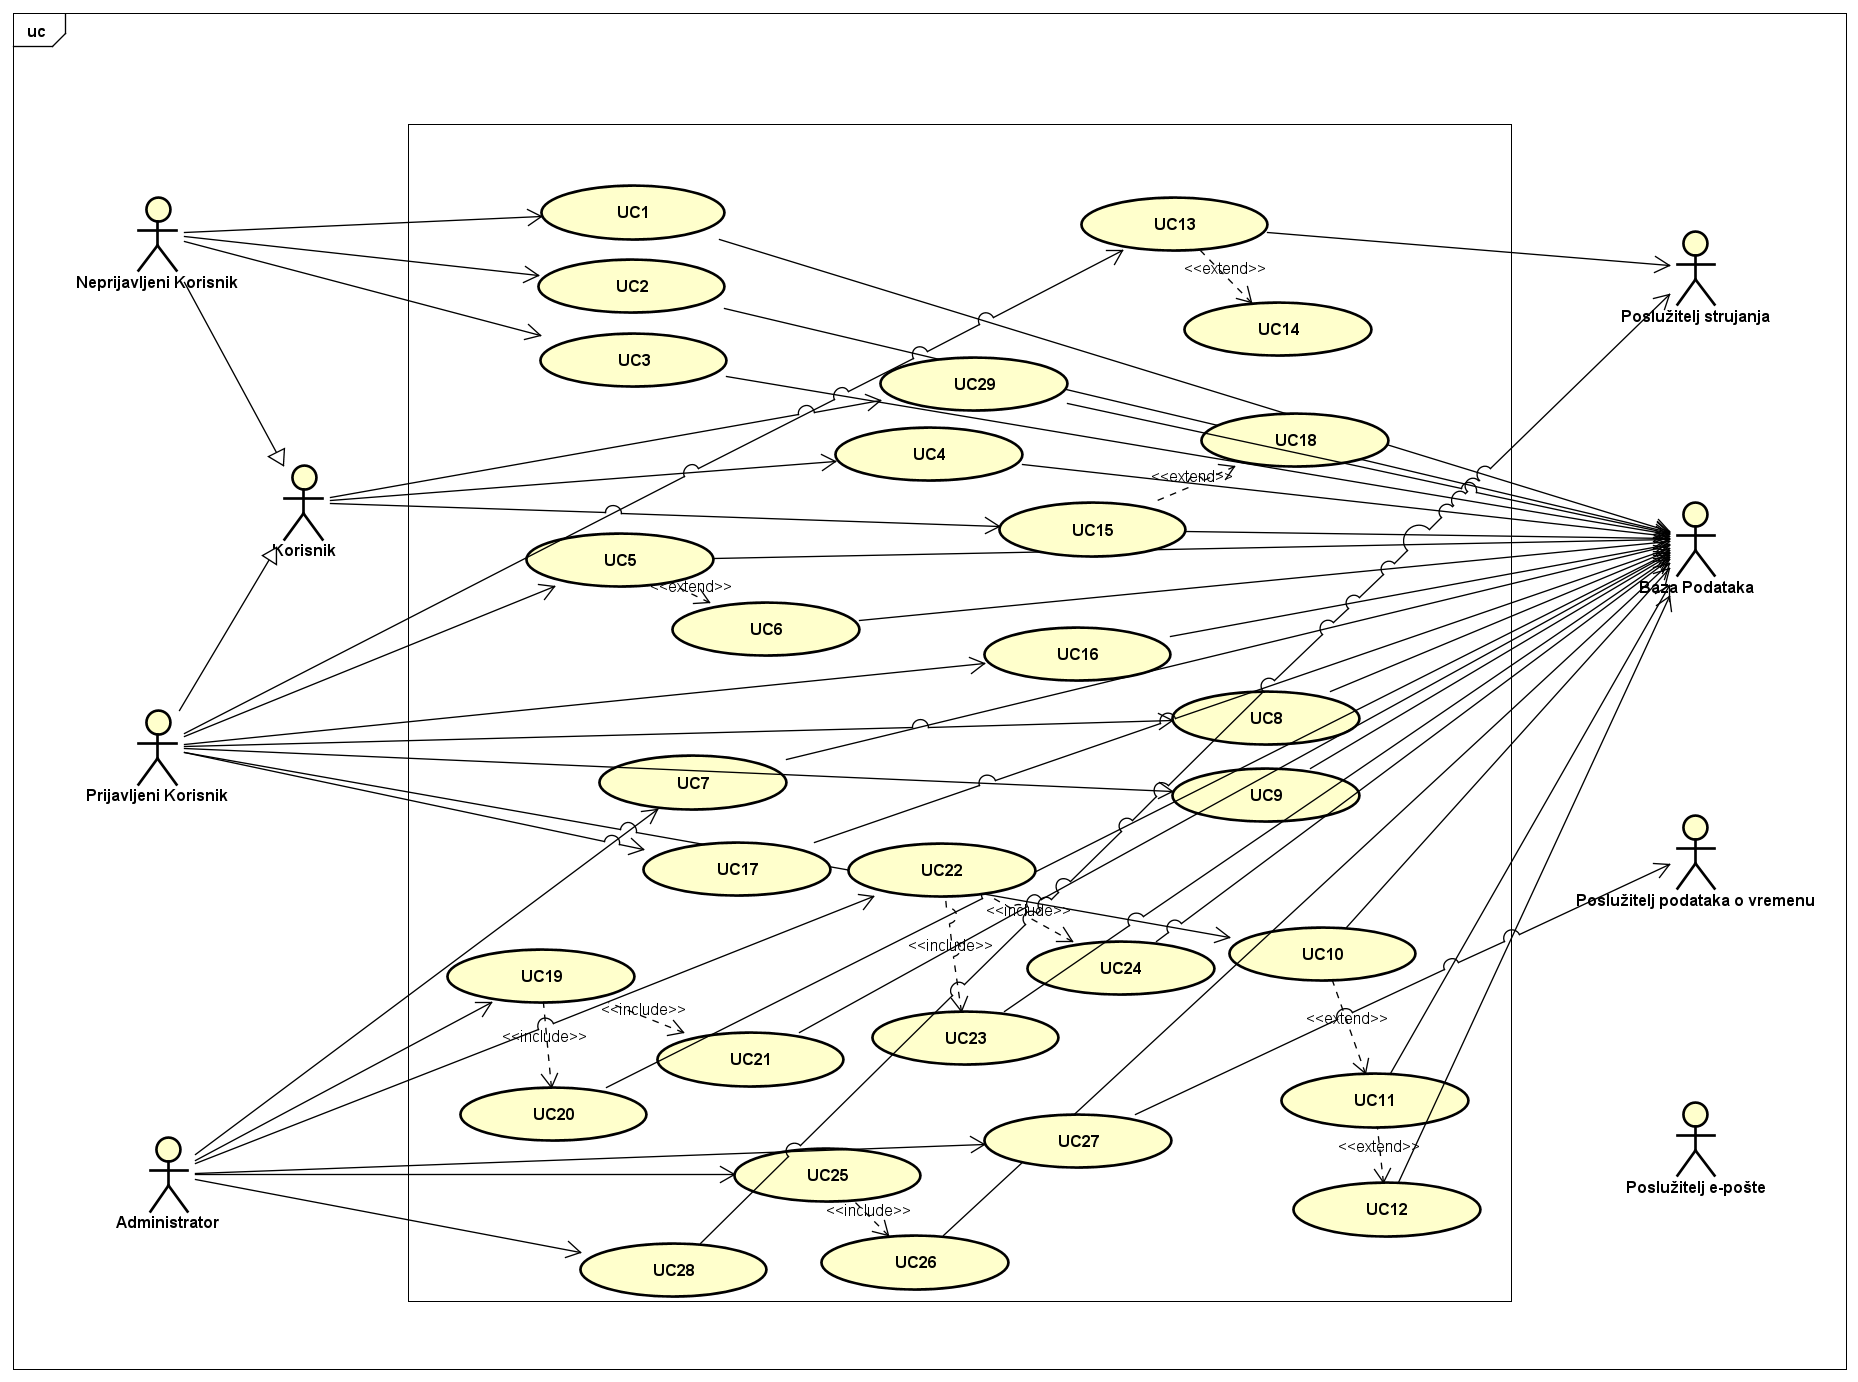
\includegraphics[width=\linewidth]{UseCaseDiagram.png}
						\caption{Početni dijagram obrazaca uporabe}
					\end{figure}
				\eject		
				
			\subsection{Sekvencijski dijagrami}
				
				\textbf{\textit{dio 1. revizije}}\\
				
				\textit{Nacrtati sekvencijske dijagrame koji modeliraju najvažnije dijelove sustava (max. 4 dijagrama). Ukoliko postoji nedoumica oko odabira, razjasniti s asistentom. Uz svaki dijagram napisati detaljni opis dijagrama.}
				\eject
	
		\section{Ostali zahtjevi}
		
			\textbf{\textit{dio 1. revizije}}\\
		 
			 \textit{Nefunkcionalni zahtjevi i zahtjevi domene primjene dopunjuju funkcionalne zahtjeve. Oni opisuju \textbf{kako se sustav treba ponašati} i koja \textbf{ograničenja} treba poštivati (performanse, korisničko iskustvo, pouzdanost, standardi kvalitete, sigurnost...). Primjeri takvih zahtjeva u Vašem projektu mogu biti: podržani jezici korisničkog sučelja, vrijeme odziva, najveći mogući podržani broj korisnika, podržane web/mobilne platforme, razina zaštite (protokoli komunikacije, kriptiranje...)... Svaki takav zahtjev potrebno je navesti u jednoj ili dvije rečenice.}
			 \begin{itemize}
			 	\item Maksimalni broj glasovanja po osobi je 1
			 	\item Glasovanje je moguće samo tijekom određenog vremenskog razdoblja koje je određeno danima i vremenom održavanja konferencije
			 \end{itemize}
			 
			 
			 
	